\documentclass{article}
\usepackage[left=2cm,right=2cm,top=2cm,bottom=2cm]{geometry}
\usepackage{tikz,pgfplots,float}
%\usetikzlibrary{tkzgraph}
\pgfplotsset{width=7cm,compat=newest}
\title{Introduction to \LaTeX{} Drawing}
\author{Siju Swamy}
\begin{document}
\maketitle
\section{Introduction}
TikZ, a high-level interface to PGF, is a language-based tool for specifying graphics. It uses familiar graphics-related concepts, such as point, line, and circle and has a concise and natural syntax. It meshes well with pdfLATEX in the sense that no additional processing steps are needed. Another positive aspect of TikZ isits ability to blend \TeX{} fonts, symbols, and mathematics within the generated graphics. TikZ supports both plain TEX and LATEX input formats and is capable of producing
PDF, PostScript, and SVG outputs. However, we limit our discussion to one
choice: \LaTeX{} input, with PDF output, processed by pdfLATEX.
TikZ provides a one-step approach to adding graphics to a \LaTeX{} document.
TikZ commands which describe the desired graphics are simply intermingled
with the text. Processing the input source yields the PDF output.

Visualization of data is often necessary and convenient in order to analyze and communicate results of
research, theses, or perhaps just results.
pgfplots is a visualization tool. The motivation for pgfplots is that you as end–user provide the data
and the descriptions as input, and pgfplots takes care of rest such as choosing suitable scaling factors,
scaling to a prescribed target dimension, choosing a good displayed range, assigning tick positions, drawing
an axis with descriptions placed at appropriate places.
pgfplots is a solution for an old problem of visualization in \LaTeX{}: its descriptions use the same fonts
as the embedding text, with exactly the same font sizes. Its direct embedding in \LaTeX{} makes the use
of \LaTeX{}’s powerful math mode as easy as possible: for any kind of axis descriptions up to user–defined
annotations. It features document–wide line–styles, color schemes, markers... all that makes up consistency.
pgfplots offers high–quality. At the same time, it is an embedded solution: it is largely independent of
3rd party–tools, although it features import functions to benefit from available tools.
Its main goal is: you provide your data and your descriptions – and pgfplots runs without more input.
If you want, you can customize what you want.

\section{Basic Settings}
To get started with TikZ we need to load up the `tikz` package in the document preamble:
\begin{verbatim}
    \usepackage{tikz}

\end{verbatim}
Now whenever we want to create a TikZ diagram we need to use the tikzpicture environment.
\begin{verbatim}

\begin{tikzpicture}
<code goes here>
\end{tikzpicture}
\end{verbatim}
As an example see the first sample code to create a line segment connecting two points:\\
\begin{figure}[H]
    \centering
    \begin{tikzpicture}
\draw (0,0) -- (1,0)-- (1,1) --(2,1);
\end{tikzpicture}
    \caption{A simple connected path}
    \label{fig:my_label}
\end{figure}

A vertical line joining with initial horizontal line can be generated as

\begin{figure}[H]
    \centering
    \begin{tikzpicture}
\draw (0,0) -|(1,1);
\end{tikzpicture}
    \caption{A simple connected vertical line}
    \label{fig:my_label}
\end{figure}

A horizontal line joining with initial vertical line can be generated as

\begin{figure}[H]
    \centering
    \begin{tikzpicture}
\draw (0,0) |- (1,1);
\end{tikzpicture}
    \caption{Another simple connected vertical line}
    \label{fig:my_label}
\end{figure}
A more general path with more connected points is shown bellow:
\begin{figure}[H]
    \centering
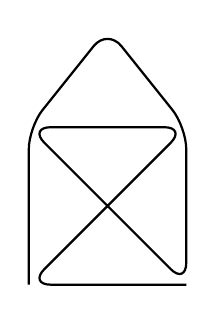
\begin{tikzpicture}
\draw[thick,rounded corners=8pt](0,0)-- (0,2)-- (1,3.25)-- (2,2)-- (2,0)-- (0,2)-- (2,2)-- (0,0)-- (2,0);
\end{tikzpicture}    \caption{A More complicated Path}
    \label{fig:my_label}
\end{figure}


\subsection{Using `pgfplots' to create plots of math functions}
pgfplots is compatible with LATEX, ConTeXt and plain \TeX{}. The only difference is how to specify environments. This affects any pgf/TikZ-environments and all pgfplots-environments like axis, semilogxaxis,
semilogyaxis and loglogaxis:

A simple example of drawing the plot of the function $y=4-x^2$ is shown bellow:

\begin{figure}[htp]
    \centering
\begin{tikzpicture}
  \begin{axis}[domain=-2:2,xlabel=$x$, ylabel={$y=4-x^2$}]
    \addplot[color=red,no marks] {4-x^2};
  \end{axis}
\end{tikzpicture} 
\caption{Graph of $y=4-x^2$}
\label{fig:my_label}
\end{figure}

We can create plots using respective coordinates as follows:
\begin{figure}[H]
    \centering
    \begin{tikzpicture}
\begin{axis}[
xlabel=Cost,
ylabel=Error]
\addplot[color=red,mark=x] coordinates {
(2,-2.8559703)
(3,-3.5301677)
(4,-4.3050655)
(5,-5.1413136)
(6,-6.0322865)
(7,-6.9675052)
(8,-7.9377747)
};
\end{axis}
\end{tikzpicture}
    \caption{Plotting Cost Vs Error}
    \label{fig:my_label}
\end{figure}

\subsection{Plotting scientific data from external files}
Here we create plots from multiple data files using pgfplot.

\begin{figure}[H]
    \centering
    \begin{tikzpicture}
\begin{loglogaxis}[
title=Convergence Plot,
xlabel={Degrees of freedom},
ylabel={$L_2$ Error},
grid=major,
legend entries={$d=1$,$d=2$,$d=3$},
]
\addplot table {data1.dat};
\addplot table {data2.dat};
\addplot table {data3.dat};
\end{loglogaxis}
\end{tikzpicture}
    \caption{Data plots from external tables}
    \label{fig:my_label}
\end{figure}
We can use external functions to calculate math functions. For example the gnuplot is the famous plotting calculator that can be used with the pgfplots.

\begin{figure}[H]
    \centering
    \begin{tikzpicture}
\begin{axis}[xlabel=$x$,ylabel=$\sin(x)$]
% invoke external gnuplot as calculator:
\addplot gnuplot[color=blue,id=sin]{sin(x)};
\end{axis}
\end{tikzpicture}
    \caption{Plot of $sin(x)$ using the gnuplot}
    \label{fig:sinplot}
\end{figure}
\subsection{Multiple plots on same axis}
We need comparative plots for various occasions. Multiple \verb+\addplot[]{}+ command will be used for this purpose. An example is shown below:

\begin{figure}[H]
    \centering
    \begin{tikzpicture}
\begin{axis}[height=9cm,width=9cm,grid=major,]
\addplot gnuplot[id=filesuffix]{(-x**5 - 242)};
\addlegendentry{model}
\addplot coordinates {
(-4.77778,2027.60977)
(-3.55556,347.84069)
(-2.33333,22.58953)
(-1.11111,-493.50066)
(0.11111,46.66082)
(1.33333,-205.56286)
(2.55556,-341.40638)
(3.77778,-1169.24780)
(5.00000,-3269.56775)
};
\addlegendentry{estimate}
\end{axis}
\end{tikzpicture}
    \caption{Multiple plots in the same axis}
    \label{fig:my_label}
\end{figure}
\subsection{Multiple plots side to side}
\begin{figure}[H]
    \centering
\begin{tikzpicture}[baseline]
\begin{axis}[
axis lines=left,
scaled ticks=false,
xticklabel style={
rotate=90,
anchor=east,
/pgf/number format/precision=3,
/pgf/number format/fixed,
/pgf/number format/fixed zerofill,
},
title=Inv. cum. normal,
xlabel={$x$},
ylabel={$y$},
ymin=-3, ymax=3,
minor y tick num=1,
]
\addplot[blue] table {invcum.dat};
\end{axis}
\end{tikzpicture}%
%
\hskip 10pt % insert a non-breaking space of specified width.
\begin{tikzpicture}[baseline]
\begin{axis}[
axis lines=left,
scaled ticks=false,
xticklabel style={
rotate=90,
anchor=east,
/pgf/number format/precision=3,
/pgf/number format/fixed,
/pgf/number format/fixed zerofill,
},
yticklabel pos=right,
]
% density of Normal distribution:
\newcommand\MU{0}
\newcommand\SIGMA{1e-3}
\addplot[red,domain=-3*\SIGMA:3*\SIGMA,samples=201]
{exp(-(x-\MU)^2 / 2 / \SIGMA^2) / (\SIGMA * sqrt(2*pi))};
\end{axis}
\end{tikzpicture}
\caption{Side by side plot}
\label{fig:sidebysideplot}
\end{figure}
\subsection{Scatter plots using pgf plot}
For this purpose we will pass the option `scatter' into the \verb+\addplot[]{}+ function as shown below:
\begin{figure}[H]
    \centering
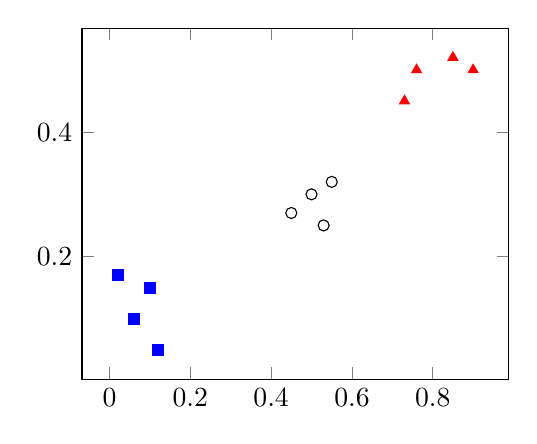
\begin{tikzpicture}
\begin{axis}
\addplot[
scatter,
only marks,
point meta=explicit symbolic,
scatter/classes={
a={mark=square*,blue},%
b={mark=triangle*,red},%
c={mark=o,draw=black}},
]
table[meta=label] {
x y label
0.1 0.15 a
0.45 0.27 c
0.02 0.17 a
0.06 0.1 a
0.9 0.5 b
0.5 0.3 c
0.85 0.52 b
0.12 0.05 a
0.73 0.45 b
0.53 0.25 c
0.76 0.5 b
0.55 0.32 c
};
\end{axis}
\end{tikzpicture}  
\caption{Scatter plot with explicit labels}
    \label{fig:my_label}
\end{figure}
\subsubsection{Scientific data plot- a case study}
The following method will plot data from three .data files available:
\begin{figure}[H]
    \centering
    
    
    \caption{Real time data plot}
    \label{fig:my_label}
\end{figure}


\subsection{Surface plots using pgf plot}
The surface plot of $z=\sin x\sin y$.
\begin{figure}[H]
    \centering
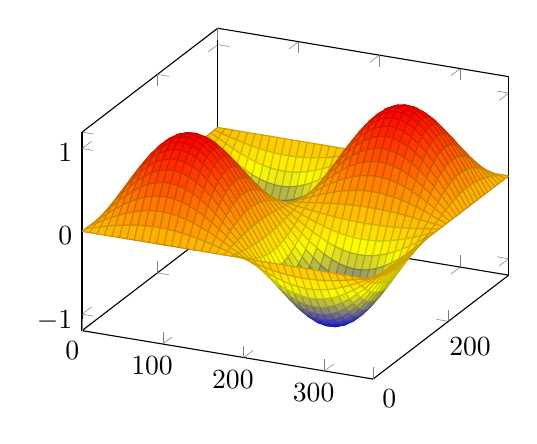
\begin{tikzpicture}
\begin{axis}
\addplot3[surf,domain=0:360,samples=40]
{sin(x)*sin(y};
\end{axis}
\end{tikzpicture}
    \caption{Plot of $z=\sin x\sin y$}
    \label{fig:my_label}
\end{figure}
\begin{figure}[H]
    \centering
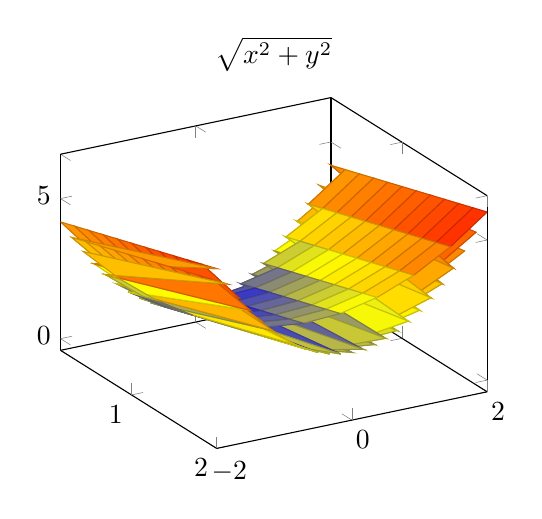
\begin{tikzpicture}
\begin{axis}[
title={$\sqrt{x^2+y^2}$},
view={60}{30},
]
\addplot3[
surf,
domain=-2:2,
domain y=-2:2,
]
{sqrt{x^2+y^2}};
\end{axis}
\end{tikzpicture}
\caption{Surface plot of $z=\sqrt{x^2+y^2}$}
    \label{fig:my_label}
\end{figure}
\begin{figure}[H]
    \centering
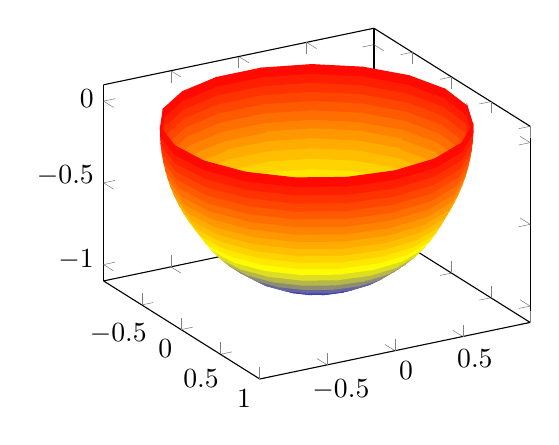
\begin{tikzpicture}
\begin{axis}[view={60}{30}]
\addplot3[surf,shader=flat,
samples=20,
domain=-1:0,y domain=0:2*pi,
z buffer=sort]
({sqrt(1-x^2) * cos(deg(y))},
{sqrt( 1-x^2 ) * sin(deg(y))},
x);
\end{axis}
\end{tikzpicture}
    \caption{Surface plot with flat shading}
    \label{fig:my_label}
\end{figure}
\begin{figure}[H]
    \centering
    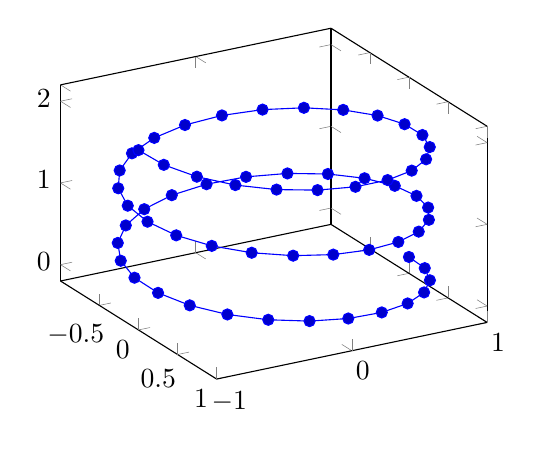
\begin{tikzpicture}
\begin{axis}[view={60}{30}]
\addplot3+[domain=0:5*pi,samples=60,samples y=0]
({sin(deg(x))},
{cos(deg(x))},
{2*x/(5*pi)});
\end{axis}
\end{tikzpicture}
    \caption{Plot of the the parametric surface $(\sin t,\cos t, 2t/5\pi)$}
    \label{fig:my_label}
\end{figure}
\subsection{Mesh plot with scatter points}
\begin{figure}[H]
    \centering
    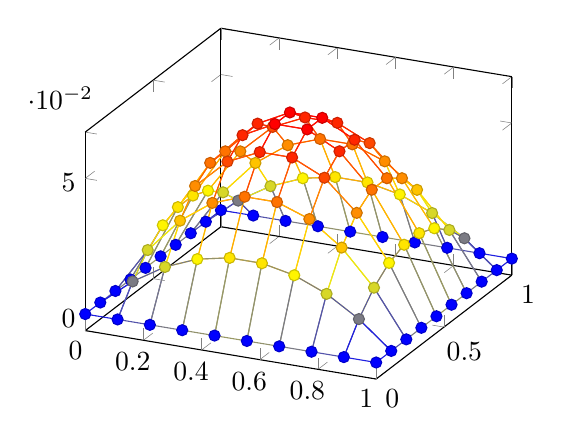
\begin{tikzpicture}
\begin{axis}
\addplot3+[mesh,scatter,samples=10,domain=0:1]
{x*(1-x)*y*(1-y)};
\end{axis}
\end{tikzpicture}
    \caption{Mesh plot with scatter points in different colours}
    \label{fig:my_label}
\end{figure}
\section{Drawing Graphs with edges and nodes- Graph theory}
%\begin{figure}[H]
%    \centering
%\begin{tikzpicture}
%\GraphInit[vstyle=Welsh]
%\SetGraphunit=2
%\Vertices={circle}{A,B,C,D,E}
%\Edges{A,B,C,D,A,C}
%\SetVertexNoLabel
%\end{tikzpicture} 
%\caption{Caption}
%    \label{fig:my_label}
%\end{figure}
\begin{figure}[H]
    \centering
   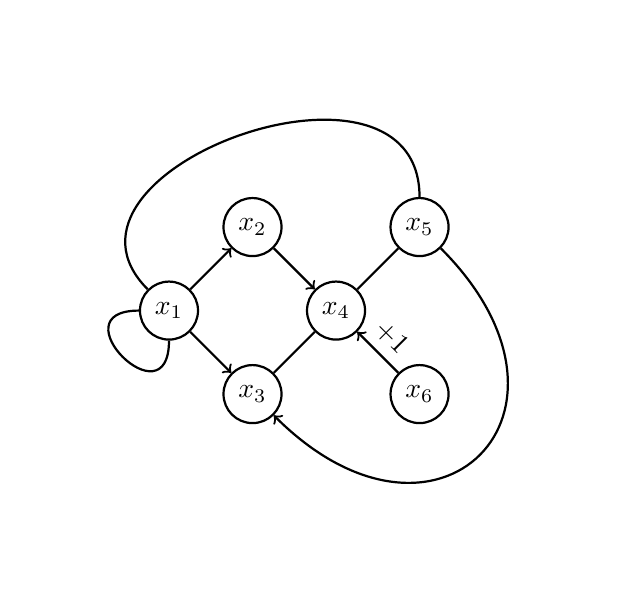
\begin{tikzpicture}[node distance={15mm}, thick, main/.style = {draw, circle}] 
\node[main] (1) {$x_1$}; 
\node[main] (2) [above right of=1] {$x_2$}; 
\node[main] (3) [below right of=1] {$x_3$}; 
\node[main] (4) [above right of=3] {$x_4$}; 
\node[main] (5) [above right of=4] {$x_5$}; 
\node[main] (6) [below right of=4] {$x_6$}; 
\draw[->] (1) -- (2); 
\draw[->] (1) -- (3); 
\draw (1) to [out=135,in=90,looseness=1.5] (5); 
\draw (1) to [out=180,in=270,looseness=5] (1); 
\draw [->](2) -- (4); 
\draw (3) -- (4); 
\draw (5) -- (4); 
\draw[->] (5) to [out=315, in=315, looseness=2.5] (3); 
\draw[->] (6) -- node[midway, above right, sloped, pos=1] {+1} (4); 
\end{tikzpicture} 
    \caption{A graph connecting nodes}
    \label{fig:my_label}
\end{figure}
\end{document}
